% seward.tex $ this file belongs to the Molcas repository $

\section{\program{seward}}
\label{UG:sec:seward}
\index{Program!Seward@\program{Seward}}\index{Seward@\program{Seward}}
%%%<MODULE NAME="SEWARD">
%%Description:
%%%<HELP>
%%+The Seward module generates one- and two-electron integrals needed
%%+by other programs. The input contains an additional and optional
%%+embedded input section for numerical quadrature options for the
%%+computation of integrals associated with DFT calculations. The
%%+embedded section starts and ends with the keywords "Grid Input"
%%+and "End of Grid", respectively. Keywords associated with this
%%+embedded input section is labelled "(NQ)" below.
%%%</HELP>
The \program{SEWARD} module generates one- and two-electron integrals needed
by other programs. The two-electron integrals may optionally be
Cholesky decomposed. In addition, it will serve as the input parser
for parameters related to the specification of the quadrature grid
used in numerical integration in association with DFT and reaction
field calculations.

%\begin{figure}
%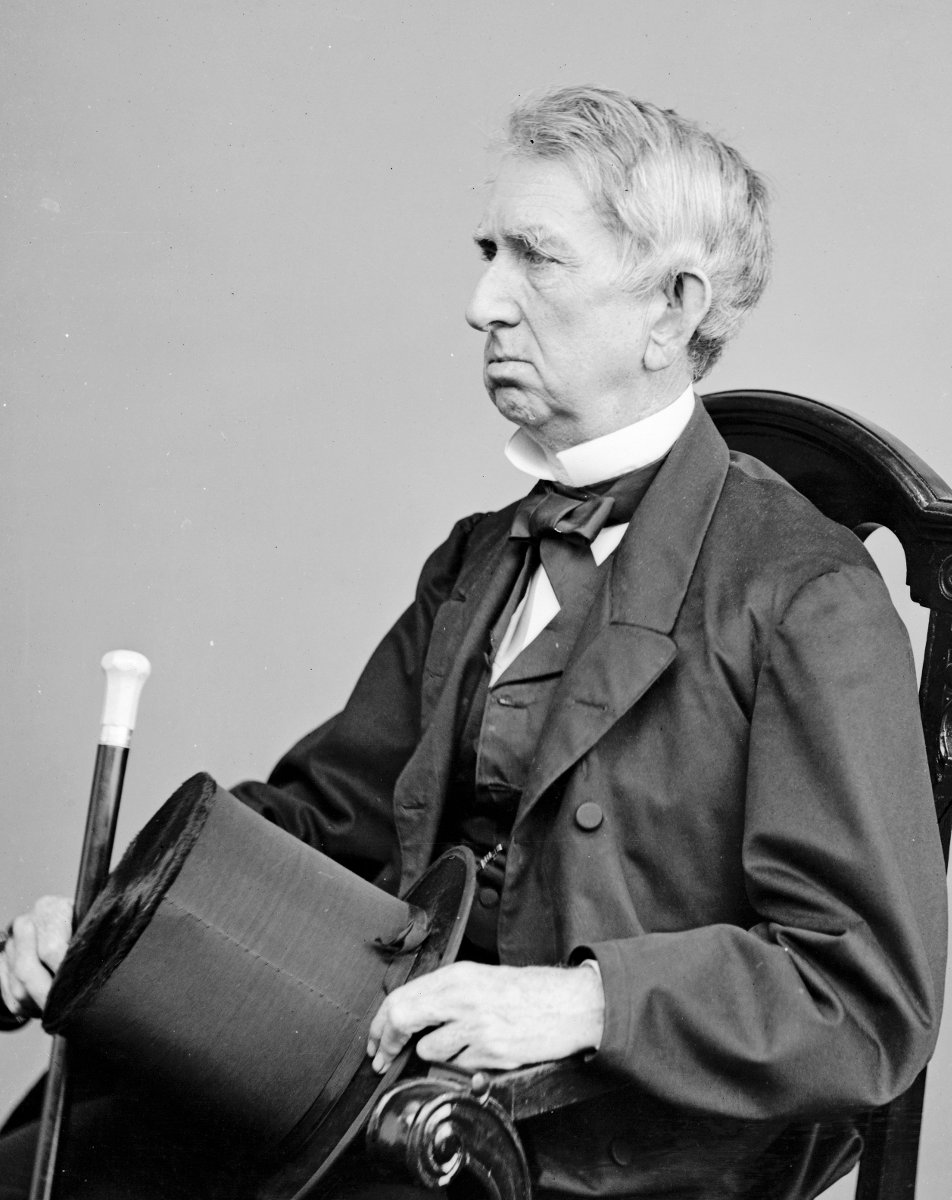
\includegraphics[scale=0.6]{users.guide/seward}
%\caption{H. W. Seward, secretary of State in the Lincoln administration, who suggested and supervised
%the 1867 purchase of Alaska from tzar Russia. Price: 2 cents an acre.}
%\end{figure}

In the following three subsection we will in detail describe the input parameters
for analytic integration, numerical integration, and reaction fields.

%\input {users.guide/integrals}
\subsection{Analytic integration}
Any conventional ab initio quantum chemical calculation starts by
computing overlap, kinetic energy, nuclear attraction and electron
repulsion integrals. These are used repeatedly to determine the
optimal wave function and the total energy of the system under
investigation. Finally, to compute various properties of the system
additional integrals may be needed, examples include multipole moments
and field gradients.

\subsubsection{Description}
\label{UG:sec:seward_description}
\program{SEWARD} is able to compute the following integrals:
\begin{itemize}
\itemsep 9pt plus 3pt minus 3pt
\item kinetic energy,
\item nuclear attraction,
\item two electron repulsion (optionally Cholesky decomposed),
\item n'th (default n=2) order moments (overlap, dipole moment, etc.),
\item electric field (generated at a given point by all charges in the system),
\item electric field gradients (spherical gradient operators),
\item linear momentum (velocity),
\item orbital angular momentum,
\item relativistic mass-{}velocity correction (1st order),
\item one-{}electron Darwin contact term,
\item one-{}electron relativistic no-pair Douglas-Kroll
\item diamagnetic shielding,
\item spherical well potential (Pauli repulsion),
\item ECP and PP integrals,
\item modified kinetic energy and multipole moment integrals
      (integration on a finite sphere centered at the origin) for use in
      the variational R-matrix approach,
\item external field (represented by a large number of charges and dipoles),
\item angular momentum products, and
\item atomic mean-field integrals (AMFI) for spin-orbit coupling.
\end{itemize}
{\it Note that while \program{SEWARD} compute these integrals the input to
select them and their settings are put in the input of \program{GATEWAY}.}

In general these integrals will be written to a file, possibly in
the form of Cholesky vectors (two-electron integrals only). However,
\program{SEWARD} can also compute the orbital contributions and total components of
these properties if provided with orbital coefficients and
orbital occupation numbers.

To generate the one-{} and two-{}electron integrals
\program{SEWARD} uses two different integration schemes. Repulsion type integrals (two-{}
electron integrals, electric field integrals, etc.) are evaluated by
the reduced multiplication scheme of the Rys quadrature \cite{seward}.
All other integrals are computed by the Gauss-Hermite quadrature.
\program{SEWARD} use spherical Gaussians as basis functions,
the only exception to this are the diffuse/polarization functions
of the 6-31G family of basis sets.
The double coset \cite{dcf} formalism is used to treat symmetry.
\program{SEWARD} is especially designed to handle ANO-{}type basis sets, however, segmented basis
sets are also processed.

At present the following limitations are built into \program{SEWARD}:

% limitations.tex $ this file belongs to the Molcas repository $*/
\bigskip\centerline{
\begin{tabular}{|lr|} \hline
{Max number of unique basis functions:}&{2000} \\
{Max number of symmetry independent centers:}\hfill&{500} \\
{Highest angular momentum:}&{15} \\
{Highest symmetry point group:}&{$D_{2h}$} \\ \hline
\end{tabular}}\bigskip


\subsubsection{Dependencies}
\label{UG:sec:seward_dependencies}
\program{SEWARD} usually runs after program \program{GATEWAY}. In the same time, any input used
in \program{GATEWAY} can be placed into \program{SEWARD} input. However, it is recommended to
specify all information about the molecule and the basis set in \program{GATEWAY} input.

\program{SEWARD} does normally not depend on any other code, except of \program{GATEWAY}.
There are two exceptions however.
The first one is when \program{SEWARD} is used as a property module. In these cases the file
\file{INPORB} has to have been generated by a wave function code. The second case, which is
totally transparent to the user, is when \program{SEWARD} picks up the new Cartesian coordinates
generated by \program{SLAPAF} during a geometry optimization.


\subsubsection{Files}
\label{UG:sec:seward_files}
\paragraph{Input Files}

Apart form the standard input file
\program{SEWARD} will use the following input files: \file{RYSRW}, \file{ABDATA},
\file{RUNFILE}, \file{INPORB} (for calculation of properties) (\ref{UG:sec:files_list}).
In addition, \program{SEWARD} uses the following files:
\begin{filelist}
%------
\item[BASLIB]
The default directory for one-particle basis set information.
This directory contains files which are part
of the program system and could
be manipulated by the user in accordance with the instructions in the
section \ref{UG:sec:the_basis_set_libraries} and following subsections.
New basis set files can be added to this directory by the local
\molcas\ administrator.
%------
\item[QRPLIB]
Library for numerical mass-velocity plus Darwin potentials (used for ECPs).
\end{filelist}

\paragraph{Output files}

In addition to the standard output file
\program{SEWARD} may generate the following files:
\file{ONEINT}, \file{ORDINT}, \file{CHVEC}, \file{CHRED}, \file{CHORST},
\file{CHOMAP}, \file{CHOR2f} (\ref{UG:sec:files_list}).

%---------------------------------------------------------------------------------

\subsubsection{Input}
\label{UG:sec:seward_input}
Below follows a description of the input to \program{SEWARD}.
Observe that if
nothing else is requested
\program{SEWARD} will by default compute the overlap, the
dipole, the quadrupole, the nuclear attraction, the kinetic energy,
the one-{}electron Hamiltonian, and the two-{}electron repulsion
integrals.

The input for each module is preceded by its name like:
\begin{inputlisting}
 &SEWARD
\end{inputlisting}

Argument(s) to a keyword, either individual or composed by several entries,
can be placed in a separated line or in the same line separated by a semicolon.
If in the same line, the first argument requires an equal sign after the
name of the keyword.

\paragraph{General keywords}
\begin{keywordlist}
%---
%%%<KEYWORD MODULE="SEWARD" NAME="TITL" APPEAR="Title (optional)" KIND="STRING" LEVEL="BASIC">
\item[TITLe]
%%%<HELP>
%%+Enter one optional title cards.
%%%</HELP>
%%%</KEYWORD>
%%Keyword: Title <basic>
%%+One line of title card follows.
One line of title card follows.
%---
\item[TEST]
%%%<KEYWORD MODULE="SEWARD" NAME="TEST" APPEAR="Test (optional)" KIND="SINGLE" LEVEL="BASIC">
%%Keyword: Test <basic>
%%%<HELP>
%%+SEWARD will only process the input and generate a non-zero
%%+return code.
%%%</HELP>
\program{SEWARD} will only process the input and generate a non-zero return code.
%%%</KEYWORD>
%---
\item[ONEOnly]
%%%<KEYWORD MODULE="SEWARD" NAME="ONEO" APPEAR="Only 1-el. Integrals (optional)" KIND="SINGLE" LEVEL="BASIC">
%%Keyword: Oneonly <basic>
%%%<HELP>
%%+SEWARD will not compute the two-electron integrals.
\program{SEWARD} will not compute the two-{}electron integrals.
%%%</HELP>
%%%</KEYWORD>
%---
\item[NODKroll]
%%%<KEYWORD MODULE="SEWARD" NAME="NODK" APPEAR="Skip Douglas-Kroll Integrals (optional)" KIND="SINGLE" LEVEL="BASIC">
%%Keyword: NoDK <basic>
%%%<HELP>
%%+SEWARD will not compute Douglas-Kroll integrals.
\program{SEWARD} will not compute Douglas-Kroll integrals.
%%%</HELP>
%%%</KEYWORD>
%---
\item[DIREct]
%%%<KEYWORD MODULE="SEWARD" NAME="DIRE" APPEAR="Direct option (optional)" KIND="SINGLE" LEVEL="BASIC">
%%Keyword: Direct <basic>
%%%<HELP>
%%+Prepares for later integral-direct calculations. As with keyword
%%+oneonly, SEWARD will evaluate no two-electron integrals.
%%%</HELP>
Prepares for later integral-{}direct calculations. As with keyword
\keyword{OneOnly}, \program{SEWARD} will evaluate no two-{}electron integrals.
%%%</KEYWORD>
%---
\item[EXPErt]
%%%<KEYWORD MODULE="SEWARD" NAME="EXPE" APPEAR="Expert mode" KIND="SINGLE" LEVEL="ADVANCED">
%%%<HELP>
%%+Activates expert mode which will deactivate some checks. This will, for
%%+example, allow the used to combine relativistic and non-relativistic basis sets.
%%%</HELP>
%%Keyword: Expert <advanced>
%%+Sets "expert mode", in which various default settings are
%%+altered. Integral-direct calculations will be carried out
%%+if the two-electron integral file is unavailable.
Sets ``expert mode'', in which various default settings are
altered. Integral-{}direct calculations will be carried out
if the two-{}electron integral file is unavailable.
%%%</KEYWORD>
%---
%%%<GROUP MODULE="SEWARD" KIND="BOX" NAME="AUX" APPEAR="CD options (optional)" LEVEL="BASIC">
%---
\item[CHOLesky]
%%%<KEYWORD MODULE="SEWARD" NAME="CHOL" APPEAR="Cholesky" KIND="SINGLE" EXCLUSIVE="RIJ,RIJK,RIC,RICD,LOW,MEDI,HIGH" LEVEL="BASIC">
%%Keyword: Cholesky <basic>
%%%<HELP>
%%+Cholesky decompose the two-electron integrals using default settings.
%%%</HELP>
\program{SEWARD} will Cholesky decompose the two-{}electron integrals using
default configuration (in particular, the decomposition threshold is
1.0d{}-4) of the decomposition driver.
The decomposition threshold can be changed using keyword \keyword{THRC}.
Default is to not decompose.
%%%</KEYWORD>
%---
\item[1CCD]
%%%<KEYWORD MODULE="SEWARD" NAME="1CCD" APPEAR="1CCD" KIND="SINGLE" LEVEL="BASIC">
%%Keyword: 1CCD <basic>
%%%<HELP>
%%+One-center Cholesky decomposition of the two-electron integrals.
%%%</HELP>
\program{SEWARD} will Cholesky decompose the two-{}electron integrals using
the one-center approximation.
The decomposition threshold can be changed using keyword \keyword{THRC}.
Default is to not decompose.
%%%</KEYWORD>
%---
\item[THRCholesky]
%%%<KEYWORD MODULE="SEWARD" NAME="THRC" APPEAR="ThrCholesky" KIND="REAL" LEVEL="BASIC">
%%Keyword: ThrCholesky <basic>
%%%<HELP>
%%+Specify decomposition threshold for Cholesky decomposition of two-electron integrals.
%%%</HELP>
Specify decomposition threshold for Cholesky decomposition of two-{}electron integrals
on the next line. Default value: 1.0d{}-4.
%%%</KEYWORD>
%---
\item[SPAN]
%%%<KEYWORD MODULE="SEWARD" NAME="SPAN" APPEAR="Span factor" KIND="REAL" LEVEL="BASIC">
%%Keyword: Span <basic>
%%%<HELP>
%%+Specify span factor (in between, but not equal to, 0 and 1) for Cholesky decomposition of two-electron integrals on the next line.
%%%</HELP>
Specify span factor ($0 < \mbox{span} \leq 1$) for Cholesky decomposition of two-electron integrals on the next line.
Span=1 implies full pivoting, Span=0 means no pivoting. If the span factor is too low, numerical errors may cause
negative diagonal elements and force the program to quit; if the span factor is too large, the execution time may
increase. Default value: 1.0d{}-2.
%%%</KEYWORD>
%---
\item[LOW Cholesky]
%%%<KEYWORD MODULE="SEWARD" NAME="LOW" APPEAR="Low" KIND="SINGLE" EXCLUSIVE="RIJ,RIJK,RIC,RICD,CHOL,MEDI,HIGH" LEVEL="BASIC">
%%Keyword: Low <basic>
%%%<HELP>
%%+Cholesky decompose the two-electron integrals using low accuracy settings. Recommended.
%%%</HELP>
\program{SEWARD} will Cholesky decompose the two-{}electron integrals using
low accuracy (threshold 1.0d{}-4)
configuration of the decomposition driver.
Default is to not decompose.
%%%</KEYWORD>
%---
\item[MEDIum Cholesky]
%%%<KEYWORD MODULE="SEWARD" NAME="MEDI" APPEAR="Medium" KIND="SINGLE" EXCLUSIVE="RIJ,RIJK,RIC,RICD,CHOL,LOW,HIGH" LEVEL="BASIC">
%%Keyword: Medium <basic>
%%%<HELP>
%%+Cholesky decompose the two-electron integrals using medium accuracy settings.
%%%</HELP>
\program{SEWARD} will Cholesky decompose the two-{}electron integrals using
medium accuracy (threshold 1.0d{}-6)
configuration of the decomposition driver.
Default is to not decompose.
%%%</KEYWORD>
%---
\item[HIGH Cholesky]
%%%<KEYWORD MODULE="SEWARD" NAME="HIGH" APPEAR="High" KIND="SINGLE" EXCLUSIVE="RIJ,RIJK,RIC,RICD,CHOL,LOW,MEDI" LEVEL="BASIC">
%%Keyword: High <basic>
%%%<HELP>
%%+Cholesky decompose the two-electron integrals using high accuracy settings.
%%%</HELP>
\program{SEWARD} will Cholesky decompose the two-{}electron integrals using
high-accuracy (threshold 1.0d-8)
configuration of the decomposition driver.
Default is to not decompose.
%%%</KEYWORD>
%---
\item[LDF]
%%%<KEYWORD MODULE="SEWARD" NAME="LDF" APPEAR="Local Density Fitting" KIND="SINGLE" EXCLUSIVE="CHOL,LOW,MEDI,HIGH" LEVEL="BASIC">
%%Keyword: LDF <basic>
%%%<HELP>
%%+Local Density Fitting using auxiliary functions centered on the two parent atoms of each AO product.
%%%</HELP>
Local Density Fitting: \program{SEWARD} will fit each AO product using only auxiliary functions centered on the two parent atoms.
Fitting coefficients are computed and stored for use in later modules (only non-hybrid KS-DFT at the moment).
Requires an auxiliary basis set (generated by RICD in Gateway or externally defined).
Can not be combined with Cholesky and (global) DF/RI. LDF is turned off by default.
%%%</KEYWORD>
%---
\item[LDF1]
%%%<KEYWORD MODULE="SEWARD" NAME="LDF1" APPEAR="Local Density Fitting" KIND="SINGLE" EXCLUSIVE="CHOL,LOW,MEDI,HIGH" LEVEL="BASIC">
%%Keyword: LDF1 <basic>
%%%<HELP>
%%+Local Density Fitting using auxiliary functions centered on the two parent atoms of each AO product. Equivalent to keyword LDF.
%%%</HELP>
Local Density Fitting using auxiliary functions centered on the two parent atoms of each AO product. Equivalent to keyword LDF.
Equivalent to keyword LDF.
%%%</KEYWORD>
%---
\item[LDF2]
%%%<KEYWORD MODULE="SEWARD" NAME="LDF2" APPEAR="Local Density Fitting with two-center auxiliary functions" KIND="SINGLE" EXCLUSIVE="CHOL,LOW,MEDI,HIGH" LEVEL="BASIC">
%%Keyword: LDF2 <basic>
%%%<HELP>
%%+Local Density Fitting using auxiliary functions centered on the two parent atoms of each AO product as well as the two-center functions required to achieve the given target accuracy.
%%%</HELP>
LDF using auxiliary functions centered on the two parent atoms of each AO product as well as the two-center functions required to achieve the given target accuracy.
%%%</KEYWORD>
%---
\item[TARGet accuracy]
%%%<KEYWORD MODULE="SEWARD" NAME="TARG" APPEAR="Target accuracy for LDF2" KIND="REAL" EXCLUSIVE="CHOL,LOW,MEDI,HIGH" LEVEL="BASIC">
%%Keyword: TARG <basic>
%%%<HELP>
%%+Specify the target accuracy for LDF2 on the next line. Default value: threshold used to generate the aCD or acCD auxiliary basis set (or 1.0d-4 in case of externally defined auxiliary basis sets).
%%%</HELP>
Specify the target accuracy for LDF2 on the next line. Default value: threshold used to generate the aCD or acCD auxiliary basis set
(or 1.0d{}-4 in case of externally defined auxiliary basis sets).
%%%</KEYWORD>
%---
\item[APTH]
%%%<KEYWORD MODULE="SEWARD" NAME="APTH" APPEAR="Atom pair threshold" KIND="REAL" EXCLUSIVE="CHOL,LOW,MEDI,HIGH" LEVEL="BASIC">
%%Keyword: APTH <basic>
%%%<HELP>
%%+Specify the LDF/LDF2 atom pair prescreening threshold on the next line, thus defining which atom pairs are considered significant. Default value: the target accuracy or the cutoff threshold for primitive integral evaluation, whichever is smaller.
%%%</HELP>
Specify the LDF/LDF2 atom pair prescreening threshold on the next line, thus defining which atom pairs are considered significant.
Default value: the target accuracy or the cutoff threshold for primitive integral evaluation, whichever is smaller.
%%%</KEYWORD>
%---
\item[CLDF]
%%%<KEYWORD MODULE="SEWARD" NAME="CLDF" APPEAR="Constrained LDF" KIND="INTEGER" EXCLUSIVE="CHOL,LOW,MEDI,HIGH" LEVEL="BASIC">
%%Keyword: CLDF <basic>
%%%<HELP>
%%+Constrained LDF/LDF2: specify constraint order on the next line (-1 for unconstrained, 0 for charge constraint). Default: unconstrained LDF.
%%%</HELP>
Constrained LDF/LDF2: specify constraint order on the next line (-1 for unconstrained, 0 for charge constraint). Default: unconstrained LDF.
%%%</KEYWORD>
%%%</GROUP>
%---
\item[FAKE CD/RI]
%%%<KEYWORD MODULE="SEWARD" NAME="FAKE" APPEAR="Skip CD/RI vectors generation (optional)" KIND="SINGLE" LEVEL="BASIC">
%%Keyword: FAKE <basic>
%%%<HELP>
%%+If CD/RI vectors are already available, SEWARD will not redo work!
If CD/RI vectors are already available, \program{SEWARD} will not redo work!
%%%</HELP>
%%%</KEYWORD>
%---
% \item[MOLPro]
% %%Keyword: MOLPRO <advanced>
% %%+The integrals are normalized as in the program package
% %%+MOLPRO. The default is the normalization
% %%+according to the double coset representatives (DCR) formalism
% %%+for conventional calculations; for Cholesky decomposition, the
% %%+default is the MOLECULE normalization (except when AMFI or
% %%+Douglas-Kroll is specified, where the DCR formalism is again
% %%+default).
% The integrals are normalized as in the program package
% \program{MOLPRO}. The default is the normalization
% according to the double coset representatives (DCR) formalism
% for conventional calculations; for Cholesky decomposition, the
% default is the \keyword{MOLECULE} normalization (except when AMFI or
% Douglas-Kroll is specified, where the DCR formalism is again
% default).
% %---
% \item[MOLEcule]
% %%Keyword: MOLECULE <advanced>
% %%+The integrals are normalized as in the integral program
% %%+MOLECULE. The default is the normalization
% %%+according to the double coset representatives (DCR) formalism
% %%+for conventional calculations; for Cholesky decomposition, the
% %%+default is the MOLECULE normalization (except when AMFI or
% %%+Douglas-Kroll is specified, where the DCR formalism is again
% %%+default).
% The integrals are normalized as in the integral program
% \program{MOLECULE}. The default is the normalization
% according to the double coset representatives (DCR) formalism
% for conventional calculations; for Cholesky decomposition, the
% default is the \keyword{MOLECULE} normalization (except when AMFI or
% Douglas-Kroll is specified, where the DCR formalism is again
% default).
% %---
% \item[MOLCas]
% %%Keyword: MOLCAS <advanced>
% %%+The integrals are normalized according to the double coset
% %%+representatives (DCR) formalism. This is the default
% %%+for conventional calculations; for Cholesky decomposition, the
% %%+default is the MOLECULE normalization (except when AMFI or
% %%+Douglas-Kroll is specified, where the DCR formalism is again
% %%+default).
% The integrals are normalized according to the double coset
% representatives (DCR) formalism. This is the default for
% conventional calculations. The default for Cholesky decompositions
% is the \keyword{MOLECULE} normalization (except when AMFI or
% Douglas-Kroll is specified, where the DCR formalism is again
% default).
% %---
\item[JMAX]
%%Keyword: JMAX <advanced>
%%+The integer entry on the next line is the highest rotational quantum
%%+number for which
%%+SEWARD will compute the rotational energy within the
%%+rigid rotor model. The default value is 5.
The integer entry on the next line is the highest rotational quantum
number for which
\program{SEWARD} will compute the rotational energy within the
rigid rotor model. The default value is 5.
%---
\item[SYMMetry]
See the the description in the manual for the program \program{GATEWAY}
%---
% \item[SKIP]
% %%Keyword: Skip <advanced>
% %%+The subsequent entry contains a sequence of integers, one for
% %%+each irreducible representation. By setting an integer to a nonzero
% %%+value all basis functions from the corresponding
% %%+irreducible representation will be removed.
% The subsequent entry contains a sequence of integers, one for
% each irreducible representation. By setting an integer to a nonzero
% value all basis functions from the corresponding
% irreducible representation will be removed.
% The default is to skip no basis functions.
% %---
% \item[NOTAbles]
% %%Keyword: Notables <advanced>
% %%+Indicates that no tables will be used for the the roots and weights
% %%+of the Rys polynomials. The default is to use tables.
% Indicates that no tables will be used for the the roots and weights
% of the Rys polynomials. The default is to use tables.
% This option is used to verify the data base for
% the calculation of roots and weights. Observe that the activation of
% this option will make the program perform rather slow.
% %---
\item[BASIs Set]
See the the description in the manual for the program \program{GATEWAY}
%---
\item[ZMAT]
See the the description in the manual for the program \program{GATEWAY}
\item[XBAS]
See the the description in the manual for the program \program{GATEWAY}
\item[XYZ]
See the the description in the manual for the program \program{GATEWAY}
%---
\item[NOGUessorb]
%%Keyword: NOGUESSORB
%%+Disable automatic generation of starting orbitals with the GuessOrb procedure.
Disable automatic generation of starting orbitals with the GuessOrb procedure.
%---
%%%<GROUP MODULE="SEWARD" KIND="BOX" NAME="DELOPT" APPEAR="Delete options" LEVEL="BASIC">
%...
\item[NODElete]
%%%<KEYWORD MODULE="SEWARD" NAME="NODE" APPEAR="No orbitals deleted" KIND="SINGLE" LEVEL="BASIC">
%%Keyword: NODElete
%%%<HELP>
%%+Do not delete any orbitals automatically.
%%%</HELP>
Do not delete any orbitals automatically.
%%%</KEYWORD>
%...
\item[SDELete]
%%%<KEYWORD MODULE="SEWARD" NAME="SDEL" APPEAR="S delete threshold" KIND="REAL" LEVEL="BASIC">
%%Keyword: SDELete
%%%<HELP>
%%+Set the threshold for deleting orbitals based on the eigenvalues of the overlap matrix.
%%%</HELP>
Set the threshold for deleting orbitals based on the eigenvalues of the overlap matrix.
All eigenvalues with eigenvectors below this threshold will be deleted.
If you want no orbitals deleted use keyword \keyword{NODElete}.
%%%</KEYWORD>
%...
\item[TDELete]
%%%<KEYWORD MODULE="SEWARD" NAME="TDEL" APPEAR="T delete threshold" KIND="REAL" LEVEL="BASIC">
%%Keyword: TDELete
%%%<HELP>
%%+Set the threshold for deleting orbitals based on the eigenvalues of the kinetic energy matrix.
%%%</HELP>
Set the threshold for deleting orbitals based on the eigenvalues of the kinetic energy matrix.
All eigenvalues with eigenvectors above this threshold will be deleted.
If you want no orbitals deleted use keyword \keyword{NODElete}.
%%%</KEYWORD>
%...
%%%</GROUP>
%---
%%%<GROUP MODULE="SEWARD" KIND="BOX" NAME="PROPT" APPEAR="Print options" LEVEL="BASIC">
%---
\item[ECPShow]
%%%<KEYWORD MODULE="SEWARD" NAME="ECPS" APPEAR="Print ECP info" KIND="SINGLE" LEVEL="BASIC">
%%Keyword: ECPSHOW
%%%<HELP>
%%+Force SEWARD to print ECP parameters.
%%%</HELP>
Force \program{SEWARD} to print ECP parameters.
%%%</KEYWORD>
%---
\item[AUXShow]
%%%<KEYWORD MODULE="SEWARD" NAME="AUXS" APPEAR="Print auxiliary basis info" KIND="SINGLE" LEVEL="BASIC">
%%Keyword: AUXSHOW
%%%<HELP>
%%+Force SEWARD to print auxiliary basis set parameters.
%%%</HELP>
Force \program{SEWARD} to print auxiliary basis set parameters.
%%%</KEYWORD>
%---
\item[BSSHow]
%%%<KEYWORD MODULE="SEWARD" NAME="BSSH" APPEAR="Print basis info" KIND="SINGLE" LEVEL="BASIC">
%%Keyword: BSSHOW
%%%<HELP>
%%+Force SEWARD to print basis set parameters.
%%%</HELP>
Force \program{SEWARD} to print basis set parameters.
%%%</KEYWORD>
%---
\item[VERBose]
%%%<KEYWORD MODULE="SEWARD" NAME="VERB" APPEAR="Verbose output" KIND="SINGLE" LEVEL="BASIC">
%%Keyword: Verbose
%%%<HELP>
%%+Force SEWARD to print a bit more verbose.
Force \program{SEWARD} to print a bit more verbose.
%%%</HELP>
%%%</KEYWORD>
%%%</GROUP>
% Thomas Dresselhaus
\item[EMBEdding]
%%%<KEYWORD NAME="EMBE" APPEAR="External embedding potential" KIND="BLOCK" LEVEL="ADVANCED">
%%%Keyword: Embedding
%%%<HELP>
%%%Reads in an embedding potential from a file and can output the density and ESP on a grid.
%%%</HELP>
%%%</KEYWORD>
Reads in an embedding potential from a file. It can also write out the
density and the electrostatic potential on a grid. It is a block keyword
which MUST be ended with \keyword{ENDEmbedding}.

The subkeywords are:
\begin{itemize}
\item[EMBInput]
Specifies the path to the file which contains the embedding potential
(e.g. {\tt EMBI=myEmbPot.dat}). The file contains a potential given on a grid. It
has the number of grid points in the first line. Then in five columns
data for each grid point is given (x, y, z, weight of this grid point,
value of the potential). Default is {\tt EMBPOT}.
\item[OUTGrid]
Specifies the path to a file containing a grid on which the output is
produced. It is only needed if you want to have the data on a grid different
from the one given in \keyword{EMBInput}. The columns for the potential and weights
are not needed in this file (and also not read in).
\item[WRDEnsity]
Switches on the calculation of the final electron density on a grid. The
output file path must be specified along with this keyword (e.g. {\tt WRDE=myDens.dat}).
\item[WREPotential]
Switches on the calculation of the electrostatic potential on a grid. The
output file path must be specified along with this keyword (e.g. {\tt WREP=myESP.dat}).
\item[ENDEmbedding]
Ends the \keyword{EMBEdding} section. This keyword MUST be present.
\end{itemize}
The EMBEdding feature is currently only supported by the SCF part of \molcas.
\end{keywordlist}

\paragraph{Keywords associated to one-{}electron integrals}
%%%<GROUP MODULE="SEWARD" NAME="ONE" APPEAR="1-electron Integral options" LEVEL="BASIC">
\begin{keywordlist}
%---
\item[MULTipoles]
%%%<KEYWORD MODULE="SEWARD" NAME="MULTIPOLE" APPEAR="Set Max order of Multipole Moment Integrals" KIND="INT" LEVEL="ADVANCED"
%%% DEFAULT_VALUE="2">
%%Keyword: Multipoles <basic>
%%%<HELP>
%%+Entry which specifies the highest order of the
%%+multipole for which integrals will be generated.
%%+For details consult the manual.
%%%</HELP>
%%%</KEYWORD>
Entry which specifies the highest order of the
multipole for which integrals will be generated. The default center
for the dipole moment operator is the origin.
The default center for the higher order operators is the
center of the nuclear mass.
The default is to do up to quadrupole moment integrals (2).
%---
\item[CENTer]
%%%<KEYWORD MODULE="SEWARD" KIND="REALS_COMPUTED" NAME="CENT" APPEAR="Multipole moments origins" SIZE="4" LEVEL="ADVANCED">
%%Keyword: Center <advanced>
%%%<HELP>
%%+This option is used to override the default selection of the origin
%%+of the multipole moment operators.
%%+On the first entry specify the number of such modifications.
%%+On the following entries enter first the order of the multipole moment operators
%%+followed by the coordinates of the origin of the operator.
%%%</HELP>
This option is used to override the default selection of the origin
of the multipole moment operators.
On the first entry add an integer entry specifying the number of
multipole moment operators for which the origin of expansion
will be defined.
Following this, one entry for each operator, the order of
the multipole operator and the coordinates of the center (in au) of
expansion are specified.
%%%</KEYWORD>
%---
\item[SDIPole]
%%%<KEYWORD MODULE="SEWARD" NAME="SDIPOLE" APPEAR="Velocity Integrals" KIND="SINGLE" LEVEL="ADVANCED">
%%Keyword: Sdipole <basic>
%%%<HELP>
%%+Requests computation of velocity integrals.
%%%</HELP>
%%%</KEYWORD>
Requests computation of velocity integrals.
%---
\item[RELInt]
%%%<KEYWORD MODULE="SEWARD" NAME="RELI" APPEAR="1st order rel. corr." KIND="SINGLE" LEVEL="ADVANCED">
%%Keyword: Relint <basic>
%%%<HELP>
%%+Requests the computation of mass-velocity and one-electron Darwin
%%+contact term integrals for the calculation of a first order correction
%%+of the energy with respect to relativistic effects.
%%%</HELP>
Requests the computation of mass-{}velocity and one-{}electron Darwin
contact term integrals for the calculation of a first order correction
of the energy with respect to relativistic effects.
%%%</KEYWORD>
%---
% \item[DOUGlas-kroll]
% %%Keyword: Douglas-Kroll <basic>
% %%+Explicit request that the one-electron Hamiltonian include the scalar relativistic
% %%+effects according to the so-called Douglas-Kroll transformation.
% %%+This option is automatically invoked for the ANO-RCC and ANO-DK3 basis sets.
% Explicit request that the one-electron Hamiltonian include the scalar relativistic
% effects according to the so-called Douglas-Kroll transformation.
% %---
% \item[BSSMethod]
% %%Keyword: BSSmethod <basic>
% %%+Request that the one-electron Hamiltonian include the scalar relativistic
% %%+effects according to the so-called Barysz-Sadlej-Snijders transformation.
% Request that the one-electron Hamiltonian include the scalar relativistic
% effects according to the so-called Barysz-Sadlej-Snijders transformation.
%---
%%%<SELECT MODULE="SEWARD" NAME="RXXPYY" CONTAINS="R02O02,R03O03,R04O04,R02O00,RxxPyy" LEVEL="BASIC">
\item[RXXPyy]
%%Keyword: RXXPyy <basic>
%%%<HELP>
%%+Request arbitrary scalar relativistic Douglas-Kroll-Hess (DKH) correction to the one-electron Hamiltonian
%%+and the so-called picture-change correction to the property integrals (multipole moments
%%+and electronic potential related properties).
%%+Here XX represents the order of the DKH correction to the one-electron Hamiltonian and
%%+yy the order of the picture-change correction. The character P denotes the parameterization
%%+used in the DKH procedure.
%%+The possible parametrizations P of the unitary transformation used
%%+in the DKH transformation supported by MOLCAS are:
%%+ (P=O) Optimum parametrization (OPT);
%%+ (P=E) Exponential parametrization (EXP);
%%+ (P=S) Square-root parametrization (SQR);
%%+ (P=M) McWeeny parametrization (MCW);
%%+ (P=C) Cayley parametrization (CAY).
%%+Hence, the proper keyword for the 4th order relativistically corrected one-electron
%%+Hamiltonian and 3rd order relativistically corrected
%%+property integrals in the EXP parameterization would read as R04E03. If yy is larger than XX it is set to
%%+XX. If yy is omitted it will default to same value as XX. Recommended orders and parametrization is
%%+R02O02.
%%+Since the EXP parameterization employs a fast algorithm, it is
%%+recommended for high order DKH transformation.
%%%</HELP>
%%%<!--The option "RxxPyy" is to provide the user with an entry in the input file which can be edited later on.-->
%%%<KEYWORD MODULE="SEWARD" NAME="R02O02" KIND="SINGLE" />
%%%<KEYWORD MODULE="SEWARD" NAME="R03O03" KIND="SINGLE" />
%%%<KEYWORD MODULE="SEWARD" NAME="R04O04" KIND="SINGLE" />
%%%<KEYWORD MODULE="SEWARD" NAME="R02O00" KIND="SINGLE" />
%%%<KEYWORD MODULE="SEWARD" NAME="RxxPyy" KIND="SINGLE" />
Request arbitrary scalar relativistic Douglas-Kroll-Hess (DKH) correction to the one-electron Hamiltonian
and the so-called picture-change correction to the property integrals (multipole moments
and electronic potential related properties).
Here XX represents the order of the DKH correction to the one-electron Hamiltonian and
yy the order of the picture-change correction. The character P denotes the parameterization
used in the DKH procedure.
The possible parametrizations P of the unitary transformation used
in the DKH transformation supported by \molcas\ are:
\begin{description}
\item[{\tt P=O}:] Optimum parametrization (OPT)
\item[{\tt P=E}:] Exponential parametrization (EXP)
\item[{\tt P=S}:] Square-root parametrization (SQR)
\item[{\tt P=M}:] McWeeny parametrization (MCW)
\item[{\tt P=C}:] Cayley parametrization (CAY)
\end{description}
Hence, the proper keyword for the 4th order relativistically corrected one-electron
Hamiltonian and 3rd order relativistically corrected
property integrals in the EXP parameterization would read as R04E03. If yy is larger than XX it is set to
XX. If yy is omitted it will default to same value as XX. Recommended orders and parametrization is
R02O02.
Since the EXP parameterization employs a fast algorithm, it is
recommended for high order DKH transformation.
%%%</SELECT>
%-----
\item[RX2C]
%%%<KEYWORD MODULE="SEWARD" NAME="RX2C" APPEAR="Relativistic X2C integrals" KIND="SINGLE" EXCLUSIVE="RX2C" LEVEL="BASIC">
%%Keyword: RX2C <basic>
%%%<HELP>
%%+Request the scalar relativistic X2C (eXact-two-Component) corrections to the
%%+one-electron Hamiltonian as well as the property integrals.
%%%</HELP>
Request the scalar relativistic X2C (eXact-two-Component) corrections to the
one-electron Hamiltonian as well as the property integrals.
%%%</KEYWORD>
%-----
\item[RBSS]
%%%<KEYWORD MODULE="SEWARD" NAME="RBSS" APPEAR="Relativistic BSS integrals" KIND="SINGLE" EXCLUSIVE="RBSS" LEVEL="BASIC">
%%Keyword: RBSS <basic>
%%%<HELP>
%%+Request the scalar relativistic BSS (Barysz-Sadlej-Snijders) corrections to the
%%+one-electron Hamiltonian as well as the property integrals. The non-iterative
%%+scheme is employed for the construction of BSS transformation.
%%%</HELP>
Request the scalar relativistic BSS (Barysz-Sadlej-Snijders) corrections to the
one-electron Hamiltonian as well as the property integrals. The non-iterative
scheme is employed for the construction of BSS transformation.
%%%</KEYWORD>
%-----
\item[RLOCal]
%%%<KEYWORD NAME="RLOCAL" APPEAR="Relativistic local approximation" KIND="SINGLE" LEVEL="BASIC">
%%Keyword: Rlocal <basic>
%%%<HELP>
%%+Request local approximation to the relativistic exact decoupling approaches such
%%+as X2C, BSS and DKH. This option cannot be used together with point group symmetry.
%%%</HELP>
Request local approximation to the relativistic exact decoupling approaches such
as X2C, BSS and DKH. This option cannot be used together with point group symmetry.
%%%</KEYWORD>
%-----
\item[NOAMfi]
%%%<KEYWORD MODULE="SEWARD" NAME="NOAM" APPEAR="No AMFI integrals" KIND="SINGLE" EXCLUSIVE="AMFI" LEVEL="BASIC">
%%Keyword: NOAMFI <basic>
%%%<HELP>
%%+Explicit request for no computation of atomic mean-field integrals.
%%%</HELP>
Explicit request for no computation of atomic mean-field integrals.
%%%</KEYWORD>
%-----
\item[AMFI]
%%%<KEYWORD MODULE="SEWARD" NAME="AMFI" APPEAR="AMFI integrals option" KIND="SINGLE" EXCLUSIVE="NOAM" LEVEL="BASIC">
%%Keyword: AMFI <basic>
%%%<HELP>
%%+Explicit request for the computation of atomic mean-field integrals (used in
%%+subsequent spin-orbit calculations). These integrals are computed by default for
%%+relativistic basis sets like the ANO-RCC and ANO-DK3 basis sets.
%%%</HELP>
Explicit request for the computation of atomic mean-field integrals (used in
subsequent spin-orbit calculations). These integrals are computed by default for the
ANO-RCC and ANO-DK3 basis sets.
%%%</KEYWORD>
%%%</GROUP>
%-----
\item[Grid Input]
Specification of numerical quadrature parameters, consult the numerical quadrature section of this
manual.
\end{keywordlist}


\paragraph{Additional keywords for property calculations}
\begin{keywordlist}
%---
%%%<GROUP MODULE="SEWARD" NAME="PROPERTY" APPEAR="Property calculations options" LEVEL="BASIC">
%---
\item[VECTors]
%%%<KEYWORD MODULE="SEWARD" NAME="VECT" APPEAR="Activate property calculation" KIND="SINGLE" LEVEL="BASIC">
%%Keyword: Vectors <basic>
%%%<HELP>
%%+Requests a property calculation. For this purpose an INPORB file must be available.
%%%</HELP>
Requests a property calculation. For this purpose a file,
\file{INPORB},
must be available, which contains the MO's and occupation numbers
of a wave function. A custom filename can be given with \keyword{FileOrb}.
%%%</KEYWORD>
%---
\item[FILEorb]
%%%<KEYWORD MODULE="SEWARD" NAME="FILE" APPEAR="Orbitals file" KIND="STRING" REQUIRE="VECT" LEVEL="BASIC">
%%Keyword: FileOrb <basic>
%%%<HELP>
%%+The next line specifies the filename containing the orbitals and occupation numbers
%%+from which the properties will be computed. By default a file named INPORB
%%+will be used.
%%%</HELP>
The next line specifies the filename containing the orbitals and occupation numbers
from which the properties will be computed. By default a file named \file{INPORB}
will be used.
%%%</KEYWORD>
%---
\item[ORBCon]
%%%<KEYWORD MODULE="SEWARD" NAME="ORBC" APPEAR="List Orbital contributions" KIND="SINGLE" REQUIRE="VECT" LEVEL="ADVANCED">
%%Keyword: Orbcon <advanced>
%%%<HELP>
%%+The keyword will force SEWARD to produce a list of the orbital
%%+contributions to the properties being computed. The default is to
%%+generate a compact list.
%%%</HELP>
The keyword will force \program{SEWARD}
to produce a list of the orbital
contributions to the properties being computed. The default is to
generate a compact list.
%%%</KEYWORD>
%---
\item[THRS]
%%%<KEYWORD MODULE="SEWARD" NAME="THRS" APPEAR="Property threshold" KIND="REAL" REQUIRE="ORBC" DEFAULT_VALUE="1.D-6" LEVEL="ADVANCED">
%%%<HELP>
%%+Specify the threshold for the occupation number of a orbital to allow that
%%+this orbital is included when listing orbital contributions to properties.
%%%</HELP>
%%Keyword: Thrs <advanced>
%%+The real entry on the following line specifies the threshold for
%%+the occupation number of an orbital in order for the
%%+keyword "OrbCon" option to list the contribution of that orbital to a
%%+property. The default is 1.0d-6.
The real entry on the following line specifies the threshold for
the occupation number of an orbital in order for the
\keyword{OrbCon}
option to list the contribution of that orbital to a property.
The default is 1.0d-{}6.
%%%</KEYWORD>
%---
\item[ORBAll]
%%%<KEYWORD MODULE="SEWARD" NAME="ORBA" APPEAR="List properties of all orbitals" KIND="SINGLE" REQUIRE="ORBC" LEVEL="ADVANCED">
%%Keyword: OrbAll <advanced>
%%%<HELP>
%%+Print computed properties for all orbitals (including unoccupied orbitals),
%%+and not weighted by orbital occupation numbers.
%%%</HELP>
%%+Requires "OrbCon".
When \keyword{OrbCon} is present, the keyword will force
\program{SEWARD} to produce a list of the computed properties
of all orbitals (including unoccupied orbitals), and the
properties are not weighted by orbital occupation numbers.
The total electronic and nuclear
contributions printed are the same as those printed by using
\keyword{OrbCon} without \keyword{OrbAll}.
%%%</KEYWORD>
%---
%%%</GROUP>
\end{keywordlist}


\paragraph{Keywords for two-{}electron integrals}
\begin{keywordlist}
%---
%%%<GROUP MODULE="SEWARD" NAME="2EL" APPEAR="2-electron integral options" LEVEL="BASIC">
%---
\item[NOPAck]
%%%<KEYWORD MODULE="SEWARD" NAME="NOPA" APPEAR="Unpacked 2-el. integrals" KIND="SINGLE" LEVEL="BASIC">
%%Keyword: Nopack <advanced>
%%%<HELP>
%%+The two-electron integrals will not be packed. The default is to
%%+pack the two-electron integrals.
%%%</HELP>
The two-{}electron integrals will not be packed. The default is to
pack the two-{}electron integrals.
%%%</KEYWORD>
%---
\item[PKTHre]
%%%<KEYWORD MODULE="SEWARD" NAME="PKTH" APPEAR="Packing threshold" KIND="REAL" DEFAULT_VALUE="1.0D-14" LEVEL="BASIC">
%%%<HELP>
%%+Specifies the desired accuracy for the packing algorithm.
%%%</HELP></KEYWORD>
%%Keyword: Pkthre <advanced>
%%+An entry specifies the desired accuracy for the packing
%%+algorithm, the default is 1.0d-14.
An entry specifies the desired accuracy for the packing
algorithm, the default is 1.0d-{}14.
%---
\item[STDOut]
%%Keyword: Stdout <advanced>
%%+Generate a two-electron integral file according to the standard of
%%+version 1 of MOLCAS. The default is to generate the
%%+two-electron integrals according to the standard used since version 2 of
%%+MOLCAS.
Generate a two-{}electron integral file according to the standard of
version 1 of \molcas. The default is to generate the
two-{}electron integrals according to the standard used since version 2 of
\molcas.
%---
\item[THREshold]
%%%<KEYWORD MODULE="SEWARD" NAME="THRE" APPEAR="To disk threshold" KIND="REAL" DEFAULT_VALUE="1.0D-14" LEVEL="BASIC">
%%%<HELP>
%%+Specify the threshold for writing integrals to disk.
%%%</HELP>
%%Keyword: Threshold <advanced>
%%+Threshold for writing integrals to disk follows. The default is 1.0d-14.
Threshold for writing integrals to disk follows. The default is 1.0d-{}14.
%%%</KEYWORD>
%---
\item[CUTOff]
%%%<KEYWORD MODULE="SEWARD" NAME="CUTO" APPEAR="Integral threshold" KIND="REAL" DEFAULT_VALUE="1.0D-16" LEVEL="BASIC">
%%%<HELP>
%%+Specify the threshold for ignoring the calculation of integrals based on the pair prefactors.
%%%</HELP>
%%Keyword: Cutoff <advanced>
%%+Threshold for ignoring the calculation of integrals based on the
%%+pair prefactor follows on the next line. The default is 1.0d-16.
Threshold for ignoring the calculation of integrals based on the
pair prefactor follows. The default is 1.0d-{}16.
%%%</KEYWORD>
%---
%%%</GROUP>
\end{keywordlist}

\paragraph{Keywords associated to electron-molecule scattering calculations
within the framework of the $R$-matrix method}

This section contains keyword which control the radial numerical integration
of the diffuse basis functions describing the scattered electrons in the
variational $R$-matrix approach. The activation of this option is controlled
by that the center of the diffuse basis is assigned the unique atom label DBAS.

\begin{keywordlist}
%---
\item[RMAT]
%%Keyword: RMAT <basic>
%%+Radius of the R-matrix sphere (in Bohr). This sphere is centered
%%+at the coordinate origin. Default value is set to 10 Bohr.
Radius of the $R$-matrix sphere (in Bohr). This sphere is centered at the
coordinate origin. The default is 10 Bohr.
%---
\item[RMEA]
%%Keyword: RMEA <advanced>
%%+Absolute precision in radial integration for R-matrix calculation.
%%+The default is 1d-9.
Absolute precision in radial integration.
The default is 1d-{}9.
%---
\item[RMER]
%%Keyword: RMER <advanced>
%%+Relative precision in radial integration for R-matrix calculation.
%%+The default is 1d-14.
Relative precision in radial integration.
The default is 1d-{}14.
%---
\item[RMQC]
%%Keyword: RMQC <advanced>
%%+Effective charge of the target molecule for R-matrix calculation.
%%+This is the effective charge seen by the incident electron outside
%%+of the R-matrix sphere. The default is 0d0.
Effective charge of the target molecule.
This is the effective charge seen by the incident electron outside
of the $R$-matrix sphere. The default is 0d0.
%---
\item[RMDI]
%%Keyword: RMDI <advanced>
%%+Effective dipole of the target molecule for R-matrix calculation.
%%+This is the effective dipole seen by the incident electron outside
%%+of the R-matrix sphere. The default is (0d0,0d0,0d0).
Effective dipole of the target molecule.
This is the effective dipole seen by the incident electron outside
of the $R$-matrix sphere. The default is (0d0,0d0,0d0).
%---
\item[RMEQ]
%%Keyword: RMEQ <advanced>
%%+Minimal value of the effective charge of the target molecule
%%+to be considered in R-matrix calculation. This is also the
%%+minimal value of the components of the effective dipole
%%+to be considered in R-matrix calculation. Default is 1d-8.
Minimal value of the effective charge of the target molecule
to be considered. This is also the
minimal value of the components of the effective dipole
to be considered. Default is 1d-{}8
%---
\item[RMBP]
%%Keyword: RMBP <advanced>
%%+Parameter used for test purposes in the definition of the
%%+Bloch term in R-matrix calculation. Default is 0d0.
Parameter used for test purposes in the definition of the
Bloch term. Default is 0d0.
%---
\item[CELL]
%%Keyword: CELL <advanced>
%%+Defines the three vectors of the unit cell (e1,e2,e3).
%%+The optional keyword
%%+Angstrom before the definition of vectors would read data in A.
%%+Must consist of three entries (four in the case of A) which correspond to coordinates of the vectors.
%%+All the atoms which
%%+are defined after that key are considered as the atoms of the cell.
Defines the three vectors of the unit cell ($\vec{e_1}$,$\vec{e_2}$,$\vec{e_3}$).
The optional keyword
{\it Angstrom} before the definition of vectors would read data in \AA.
Must consist of three entries (four in the case of \AA) which correspond to coordinates of the vectors. All the atoms which
are defined after that key are considered as the atoms of the cell.
%---
\item[SPREad]
%%Keyword: SPREAD <advanced>
%%+Three integer numbers n_1, n_2, n_3 which define the spread of the unit cell along the unit cell vectors.
%%+For example, 0 0 2 would add all cell's atoms translated on -2*e3, -e3, e3, 2*e3.
%%+This key must be placed before the definition of the unit cell atoms.
Three integer numbers $n_1$, $n_2$, $n_3$ which define the spread of the unit cell along the unit cell vectors.
For example, $0\quad 0\quad 2$ would add all cell's atoms translated on $-2\vec{e_3}$, $-\vec{e_3}$, $\vec{e_3}$, $2\vec{e_3}$.
This key must be placed {\bf before} the definition of the unit cell atoms.
\end{keywordlist}

Below follows an input for the calculation of integrals of a carbon
atom. The comments in the input gives a brief explanation of the
subsequent keywords.

%%%To_extract{/doc/samples/ug/SEWARD.C.input}
\begin{inputlisting}
 &SEWARD
Title= This is a test deck!
* Remove integrals from a specific irreps
Skip= 0 0 0 0 1 1 1 1
* Requesting only overlap integrals.
Multipole= 0
* Request integrals for diamagnetic shielding
DSHD= 0.0 0.0 0.0; 1; 0.0 0.0 0.0
* Specify a title card
* Request only one{-}electron integrals to be computed
OneOnly
* Specify group generators
Symmetry= X Y Z
* Enable an inline basis set
Expert
* Specify basis sets
Basis set
C.ANO-L...6s5p3d2f.
Contaminant d
C  0.0 0.0 0.0
End of basis
\end{inputlisting}
%%%To_extract

\paragraph{The basis set label and the all electron basis set library}

The label, which defines the basis set for a given atom or set of atoms,
is given as input after the
keyword \keyword{Basis set}. It has the following general
structure (notice that the last
character is a period):

\fbox{atom.type.author.primitive.contracted.aux.}

where the different identifiers have the following meaning:

\begin{whatnotlist}{\tt}{Identifier}{Meaning}
%---
\item[atom]
Specification of the atom by its chemical symbol.
%---
\item[type]
Gives the type of basis set (ANO, STO, ECP, etc.) according to
specifications given in the basis set library, {\em vide supra}.
Observe that the upper cased character of the type label
defines the file name in the basis directory.
%---
\item[author]
First author in the publication where that basis set appeared.
%---
\item[primitive]
Specification of the primitive set (e.g. 14s9p4d3f).
%---
\item[contracted]
Specification of the contracted set to be selected. Some basis
sets allow only one type of contraction, others all types up
to a maximum. The first basis functions for each angular
momentum is then used.
{\bf Note}, for the basis set types ANO and ECP, on-the-fly decontraction of the most
diffuse functions are performed in case the number of contracted functions specified in this field
exceeds what formally is specified in the library file.
%---
\item[aux]
Specification of the type of AIMP, for instance, to choose between
non-relativistic and relativistic core AIMP's.
%---
\end{whatnotlist}
Only the identifiers \verb+atom+, \verb+type+,
and \verb+contracted+ have to be included in
the label. The others can be left out. However, the periods have to be
kept. Example --- the basis set label
`\verb+C.ano-s...4s3p2d.+'
will by \molcas\ be
interpreted as
`\verb+C.ano-s.Pierloot.10s6p3d.4s3p2d.+',
which is the first
basis set in the ANO-S file in the
basis directory that fulfills the specifications given.

More information about basis set format can be found in
the section Advanced examples.

\noindent

\subsection{Numerical integration}
\label{UG:sec:dft}
\index{Numerical Integration}

Various Density Functional Theory (DFT) models can be used in \molcas\ .
Energies and analytical gradients are available for all DFT models.
In DFT the exact exchange present in HF theory is replaced by a more general
expression, the exchange-correlation functional, which accounts for both the exchange energy, E$_X [P]$
and the electron correlation energy ,E$_C [P]$.

\subsubsection{Description}
\label{UG:sec:dft_description}
We shall now describe briefly how the exchange and correlation energy terms look like.
The functionals used in DFT are integrals of some function of the electron density and optionally the gradient
of the electron density
\begin{equation}
E_X[P] = \int f(\rho_{\alpha}(r), \rho_{\beta}(r), \nabla \rho_{\alpha}(r), \nabla \rho_{\beta}(r)) dr
\end{equation}

The various DFT methods differ in which function, f, is used for E$_X[P]$ and for E$_C[P]$.
In \molcas\ pure DFT methods are supported, together with hybrid methods, in which the exchange functional
is a linear combination of the HF exchange and a functional integral of the above form.
The latter are evaluated by numerical quadrature.
In the \program{SEWARD} input the parameters for the numerical integration can be set up.
In the \program{SCF} and \program{RASSCF} inputs the keywords for
using different functionals can be specified.
Names for the various pure DFT models are given by combining the names for the exchange and correlation functionals.

The DFT gradients has been implemented for both the fixed and the moving grid approach \cite{Johnson:93,Handy:93,Baker:94}.
The latter is known to be translationally invariant by definition and is recommended in geometry optimizations.

%\subsubsection{Files}
%\label{UG:sec:dft_files}
%
%
%\begin{filelist}
%\item[RUNFILE]
%The run file will contain the parameters defining and controlling the numerical integration.
%\end{filelist}


\subsubsection{Input}

Below follows a description of the input to the numerical integration utility in the
\program{SEWARD} input.

Compulsory keywords
\begin{keywordlist}
\item[GRID Input]
This marks the beginning of the input to the numerical integration utility.
\item[END Of Grid-Input]
This marks the end of the input to the numerical integration utility.
\end{keywordlist}

%%%<GROUP MODULE="SEWARD" NAME="GRID" APPEAR="Numerical Quadrature Options" LEVEL="ADVANCED">
%%Keyword: Grid input <basic>
%%%<HELP>
%%+Specification of numerical quadrature parameters.
%%%</HELP>
Optional keywords
\begin{keywordlist}
%-------
% \item[GLOBal]
% %%Keyword: Global <advanced>
% %%+It activates the use of the global partitioning technique.
% It activates the use of the global partitioning technique.
% %-------
\item[GRID]
%%%<KEYWORD MODULE="SEWARD" NAME="GRID" APPEAR="Generic Grids" KIND="CHOICE" LEVEL="ADVANCED">
%%%LIST="FINE,COARSE,SG1GRID,ULTRAFINE">
%%Keyword: Grid (NQ) <advanced>
%%%<HELP>
%%+It specifies the quadrature quality.
%%+The possible indexes that can follow are
%%+COARSE, SG1GRID, FINE, ULTRAFINE
%%+following the Gaussian98 convention.
%%+Default is FINE.
%%%</HELP>
%%%</KEYWORD>
It specifies the quadrature quality.
The possible indexes that can follow are
COARSE, SG1GRID, FINE, ULTRAFINE
following the Gaussian98 convention.
Default is FINE.
%-------
\item[RQUAd]
%%%<KEYWORD MODULE="SEWARD" NAME="RQUA" APPEAR="Radial grid type" KIND="CHOICE" LEVEL="ADVANCED"
%%% LIST="MHL,LOG3,BECKE,TA,LMG">
%%Keyword: RQuad (NQ) <advanced>
%%%<HELP>
%%+It specifies the radial quadrature scheme.
%%+Options are LOG3 (Mura and Knowles), BECKE (Becke) , MHL (Murray et a.), TA (Treutler and
%%+Ahlrichs, defined for H-Kr), and LMG (Lindh et al.), respectively. The default is MHL.
%%%</HELP>
%%%</KEYWORD>
It specifies the radial quadrature scheme.
Options are LOG3 (Mura and Knowles)\cite{Mura:96}, BECKE
(Becke)\cite{BeckeG:88}, MHL (Murray et al.)\cite{Murray:93}, TA (Treutler and
Ahlrichs, defined for H-Kr)\cite{Treutler:95}, and LMG (Lindh et
al.)\cite{LMG:01}, respectively. The default is MHL.
%-------
%%%<KEYWORD MODULE="SEWARD" NAME="AGRID" APPEAR="Angular Grid" KIND="CHOICE" LEVEL="ADVANCED"
%%% LIST="LEBEDEV,LOBATTO,GGL">
%%%<HELP>
%%+Specifies the type of angular grid. Options are Gauss-Gauss-Legendre (GGL), Lobatto, and
%%+Lebedev. Lebedev is the default.
%%%</HELP>
%%%</KEYWORD>
%-------
\item[GGL ]
%%Keyword: GGL (NQ) <advanced>
%%+It activates the use of Gauss and Gauss-Legendre angular quadrature.
%%+Default is to use the Lebedev angular grid.
It activates the use of Gauss and Gauss-Legendre angular quadrature.
Default is to use the Lebedev angular grid.
%-------
\item[LEBEdev]
%%Keyword: Lebedev (NQ) <advanced>
%%+It turns on the Lebedev angular grid.
It turns on the Lebedev angular grid.
%-------
\item[LOBAtto]
%%Keyword: Lobatto (NQ) <advanced>
%%+It activates the use of Lobatto angular quadrature.
%%+Default is to use the Lebedev angular grid.
It activates the use of Lobatto angular quadrature.
Default is to use the Lebedev angular grid.
%-------
\item[LMAX]
%%%<KEYWORD MODULE="SEWARD" NAME="LMAX" APPEAR="Angular Grid Size" KIND="INT" DEFAULT_VALUE="29" LEVEL="ADVANCED">
%%Keyword: LMax (NQ) <advanced>
%%%<HELP>
%%+Specifies the highest order of a real spherical harmonic which the angular grid will integrate exact. Default is 29.
%%%</HELP>
%%%</KEYWORD>
It specifies the angular grid size. Default is 29.
%-------
\item[NGRId]
%%%<KEYWORD MODULE="SEWARD" NAME="NGRI" APPEAR="Batch size" KIND="INT" DEFAULT_VALUE="128" LEVEL="ADVANCED">
%%Keyword: nGrid (NQ) <advanced>
%%%<HELP>
%%+It specifies the maximum number of grid points to process at one instance.
%%+Default is 128 grid points.
%%%</HELP>
%%%</KEYWORD>
It specifies the maximum number of grid points to process at one instance.
Default is 128 grid points.
%-------
\item[NOPRunning]
%%%<KEYWORD MODULE="SEWARD" NAME="NOPR" APPEAR="No Prunning of Grid" KIND="SINGLE" LEVEL="ADVANCED">
%%Keyword: Noprunning (NQ) <advanced>
%%%<HELP>
%%+It turns off the the angular prunning. Default is to prune.
%%%</HELP>
%%%</KEYWORD>
It turns off the the angular prunning. Default is to prune.
%-------
\item[NR  ]
%%%<KEYWORD MODULE="SEWARD" NAME="NR" APPEAR="Radial Grid Size" KIND="INT" DEFAULT_VALUE="75" LEVEL="ADVANCED">
%%Keyword: nR (NQ) <advanced>
%%%<HELP>
%%+It is followed by the number of radial grid points. Default is 75 radial grid points.
%%%</HELP>
%%%</KEYWORD>
It is followed by the number of radial grid points. Default is 75 radial grid points.
%-------
% \item[WHOLe]
% %%Keyword: Whole (NQ) <advanced>
% %%+It activates the use of routines which scan the whole atomic grid for
% %%+each sub block. Default is to only scan the relevant part.
% It activates the use of routines which scan the whole atomic grid for
% each sub block. Default is to only scan the relevant part.
% %-------
%%%<KEYWORD MODULE="SEWARD" NAME="FIXE" APPEAR="Grid type" KIND="CHOICE" LEVEL="ADVANCED"
%%% LIST="MOVING,FIXED">
%%%<HELP>
%%+Specify if the grid should be fixed or moving. A moving grid is default.
%%%</HELP>
%%%</KEYWORD>
\item[FIXEd grid]
%%Keyword: Fixed Grid (NQ) <advanced>
%%+Use a fixed grid in the evaluation of the gradient. This corresponds to
%%+using the grid to numerically evaluate the analytic gradient expression.
%%+Default is to use a moving grid.
Use a fixed grid in the evaluation of the gradient. This corresponds to
using the grid to numerically evaluate the analytic gradient expression.
Default is to use a moving grid.
%-------
\item[MOVIng grid]
%%Keyword: Moving grid (NQ) <advanced>
%%+Use a moving grid in the evaluation of the gradient. This correspond to
%%+evaluating the gradient of the numerical expression of the DFT energy. This is the default.
Use a moving grid in the evaluation of the gradient. This correspond to
evaluating the gradient of the numerical expression of the DFT energy. This is the default.
%-------
\item[THREshold]
%%%<KEYWORD MODULE="SEWARD" NAME="THRE" APPEAR="Radial Grid Threshold" KIND="REAL" DEFAULT_VALUE="1.0D-13" LEVEL="ADVANCED">
%%Keyword: Threshold (NQ) <advanced>
%%%<HELP>
%%+Follows the value for the the radial threshold.
%%+Default value is 1.0D-13.
%%%</HELP>
%%%</KEYWORD>
It is followed by the value for the the radial threshold.
Default value is 1.0D{}-13.
%-------
\item[T\_X]
%%%<KEYWORD MODULE="SEWARD" NAME="T_X" KIND="REAL" DEFAULT_VALUE="1.0D-18" LEVEL="ADVANCED">
%%Keyword: T_X (NQ) <advanced>
%%%<HELP>
%%+Threshold for screening in the assembling of the density on the grid.
%%+Default value is 1.0D-18.
%%%</HELP>
%%%</KEYWORD>
Threshold for screening in the assembling of the density on the grid.
Default value is 1.0D{}-18.
%-------
\item[T\_Y]
%%%<KEYWORD MODULE="SEWARD" NAME="T_Y" KIND="REAL" DEFAULT_VALUE="1.0D-11" LEVEL="ADVANCED">
%%Keyword: T_Y (NQ) <advanced>
%%%<HELP>
%%+Threshold for screening in the assembling of the integrals.
%%+Default value is 1.0D-11.
%%%</HELP>
%%%</KEYWORD>
Threshold for screening in the assembling of the integrals.
Default value is 1.0D{}-11.
%-------
\item[NOSCreening]
%%%<KEYWORD MODULE="SEWARD" NAME="NOSC" APPEAR="NoScreening" KIND="SINGLE" LEVEL="ADVANCED">
%%Keyword: NOSCreening (NQ) <basic>
%%%<HELP>
%%+Turn off any screening in the numerical integration.
%%%</HELP>
%%%</KEYWORD>
Turn off any screening in the numerical integration.
%-------
\item[CROWding]
%%%<KEYWORD MODULE="SEWARD" NAME="CROW" APPEAR="CROWDING" KIND="REAL" DEFAULT_VALUE="3.0" LEVEL="ADVANCED">
%%Keyword: CROWding (NQ) <basic>
%%%<HELP>
%%+The crowding factor, according to MHL, used in the pruning of the angular
%%+grid close to the nuclei. Default value 3.0.
The crowding factor, according to MHL, used in the pruning of the angular
grid close to the nuclei. Default value 3.0.
%%%</HELP>
%%%</KEYWORD>
\end{keywordlist}
%%%</GROUP>

The \program{SCF} and \program{RASSCF} programs have
their own keywords to decide which functionals to use in a DFT calculation.

Below follows an example of a DFT calculation with two different functionals.

%%%To_extract{/doc/samples/ug/DFT.H.input}
\begin{inputlisting}
 &GATEWAY
Basis set
H.3-21G.....
H1 0.0  0.0 0.0
End of basis

 &SEWARD
Grid input
 RQuad= Log3; nGrid= 50000; GGL; lMax= 26; Global
End of Grid Input

 &SCF; Occupations=1; KSDFT=LDA5; Iterations= 1 1

 &SCF; Occupations= 1; KSDFT=B3LYP; Iterations= 1 1

\end{inputlisting}
%%%To_extract

\subsection{Relativistic operators}

The current different implementation of all relativistic operators in \molcas\ as
described in the following subsubsections has been programmed and tested in
Ref.\cite{R2C_review}

\subsubsection{Using the Douglas--Kroll--Hess Hamiltonian}

For all-electron calculations, the preferred way is to use the scalar-relativistic
Douglas--Kroll--Hess (DKH) Hamiltonian, which, in principle, is available up to arbitrary
order in Molcas; for actual calculations, however,
the standard 2nd order is usually fine, but one may use a higher order that 8th order
by default to be on the safe side.

The arbitrary-order Hamiltonian is activated by setting

\hspace*{1cm} {\tt RXXPyy}

somewhere in the \program{SEWARD} input, where
the {\tt XX} denotes the order of the DKH Hamiltonian in the external potential.
I.e., for the standard 2nd-order Hamiltonian you may use {\tt R02O}.
Note
in particular that the parametrization {\tt P} does not affect the Hamiltonian up to
fourth order. Therefore, as long as you run calculations with DKH Hamiltonians below
5th order you may use any symbol for the parametrization as they would all yield the
same results.

The possible parametrizations {\tt P} of the unitary transformation used
in the DKH transformation supported by \molcas\ are:
\begin{description}
\item[{\tt P=O}:] Optimum parametrization (OPT)
\item[{\tt P=E}:] Exponential parametrization (EXP)
\item[{\tt P=S}:] Square-root parametrization (SQR)
\item[{\tt P=M}:] McWeeny parametrization (MCW)
\item[{\tt P=C}:] Cayley parametrization (CAY)
\end{description}

Up to fourth order ({\tt XX=04}) the DKH Hamiltonian is independent of the chosen
parametrization.
Higher-order DKH Hamiltonians depend slightly on the chosen parametrization of the unitary
transformations applied in order to decouple the Dirac Hamiltonian.
Since the EXP parameterization employs a fast algorithm \cite{DKH_polynomial}, it is recommended
for high-order DKH transformation.

For details on the arbitrary-order DKH Hamiltonians see \cite{DKH_Theory} with respect to theory,
\cite{DKH_Implementation} with respect to aspects of implementation, and
\cite{DKH_Principles} with respect to general principles of DKH.
The current version of \molcas\ employs different algorithms,
but the polynomial cost scheme of the DKH implementation as described in \cite{DKH_polynomial} is
used as the default algorithm. The implementation in MOLCAS has been presented in \cite{R2C_review}.

For details on the different parametrizations of the unitary transformations see \cite{DKH_Parameterization}.


\subsubsection{Douglas--Kroll--Hess transformed properties}

As mentioned above, four-component molecular property operators need to be DKH
transformed as well when going from a four-component to a two- or one-component description;
the results do not coincide with the well-known corresponding nonrelativistic expressions
for a given property but are properly picture change corrected.

The transformation of electric-field-like molecular property operators can be carried
out for any order smaller or equal to the order chosen for the scalar-relativistic DKH Hamiltonian.
In order to change the default transformation of order 2, you may concatenate the
input for the DKH Hamiltonian by 2 more numbers specifying the order in the property,

\hspace*{1cm} {\tt RxxPyy}

where {\tt yy} denotes the order of the Hamiltonian starting with first order 01.
The DKH transformation is then done automatically for all one-electron electric-field-like
one-electron property matrices.

Also note that the current implementation of both the Hamiltonian and the property
operators is carried out in the full, completely decontracted basis set of the
molecule under consideration. The local nature of the relativistic contributions is not
yet exploited and hence large molecules may require considerable computing time for
all higher-order DKH transformations.

For details on the arbitrary-order DKH properties see \cite{DKH_Theory2} with respect to theory
and \cite{DKH_Implementation2,R2C_review} with respect to implementation aspects.

\subsubsection{Using the X2C/Barysz--Sadlej--Snijders Hamiltonian}

Exact decoupling of the relativistic Dirac Hamiltonian can be achieved with infinite-order
approaches, such as the so-called X2C (exact--two--component) and BSS (Barysz--Sadlej--Snijders)
method. In Molcas, both methods are available for all-electron calculations. The
evaluation of transformation matrices employs a non-iterative scheme.
%which is superior to the iterative scheme in convergence behavior and computational cost.

The exact decoupling Hamiltonian is activated by setting either {\tt RX2C} or {\tt RBSS}
somewhere in the {\tt SEWARD} input, where {\tt RX2C} and {\tt RBSS} denote using the
scalar (one-component) X2C and BSS Hamiltonian respectively. The one-electron Hamiltonian
as well as the property integrals will be transformed according to the given exact decoupling method.
In other words, all property integrals are by default picture change corrected.

The computation time of the X2C/BSS method is almost the same as of the DKH method at 8th order,
while X2C is a little bit faster than BSS since the additional free-particle Foldy--Wouthuysen
transformation is skipped in the X2C approach\cite{R2C_review}. For molecules including only light atoms,
the DKH method with low orders ($<$8) is enough to account for the relativistic effects.
%As for heavy
%elements containing molecules, DKH with low orders is not accurate enough while DKH with high
%orders is computational expensive, the X2C method is then recommended in this case.

The differences between different exact decoupling relativistic methods are very small compared
to errors introduced by other approximations, such as the basis set incompleteness, approximate
density functionals, etc. Therefore, any exact decoupling model is acceptable for the
treatment of relativistic effects in molecular calculations.

For details on the exact decoupling approaches see \cite{R2C_review} with respect to theories and
comparison of numerical results, \cite{X2C_kut05jcp,X2C_liu06jcp,X2C_pen07jcp} for the X2C method, and
\cite{BSS_bar97ijqc,BSS_ked07cpl} for the BSS method.

\subsubsection{Local approximation to relativistic decoupling}

The computational cost for relativistic transformations increases rapidly if the molecule becomes
larger. The local DLU scheme \cite{DLU_Theory} was proposed to reduce the computational cost
based on the atomic decomposition of the (unitary) decoupling transformation.  It is important to note that
the DLU scheme can be applied to any kind of relativistic approaches mentioned above (i.e., DKH, BSS, and X2C). It was found \cite{DLU_Theory}
that the DLU approximation introduces very small errors for total energies, which are less than
0.01 milli-Hartree for molecules including heavy atoms.
The local approximation is activated by setting {\tt RLOCal} somewhere in the {\tt SEWARD} input.

The direct local approximation to the Hamiltonian, called DLH in Ref.  \cite{DLU_Theory} may be activated by setting {\tt RLOCal=DLH}.
However, as DLH is not superior to the DLU scheme, but introduces slightly larger errors, it is not recommended.

The picture-change effect for molecular properties is automatically taken care of when a local approximation is employed for the transformed
operator. The default order of DKH transformed properties is set to the same as the order of the DKH Hamiltonian.

It is important to note the local approximation cannot be used together with point group symmetry
in the current implementation. Because the relativistic transformation is applied in the molecular
orbital (MO) representation instead of the atomic orbital (AO) representation. Thus, the program will
report an error and exit if symmetry is used.

%%%</MODULE>
